\documentclass[a4paper,12pt]{article}
\usepackage[utf8]{inputenc}
\usepackage[spanish]{babel}
\usepackage{amsmath}
\usepackage{amsfonts}
\usepackage{amssymb}
\usepackage{multirow}
%\usepackage{makeidx}
\usepackage{graphicx}
\usepackage{fancyhdr}
\usepackage{hyperref}
\usepackage{float}
\usepackage{color}
\definecolor{azulUC3M}{RGB}{0,0,102}
\definecolor{gray97}{gray}{.97}
\definecolor{gray75}{gray}{.75}
\definecolor{gray45}{gray}{.45}
\usepackage{listings}
\lstset{ frame=Ltb,
     framerule=0pt,
     aboveskip=0.5cm,
     framextopmargin=3pt,
     framexbottommargin=3pt,
     framexleftmargin=0.4cm,
     framesep=0pt,
     rulesep=.4pt,
     backgroundcolor=\color{gray97},
     rulesepcolor=\color{black},
     %
     stringstyle=\ttfamily,
     showstringspaces = false,
     basicstyle=\small\ttfamily,
     commentstyle=\color{gray45},
     keywordstyle=\bfseries,
     %
     numbers=left,
     numbersep=15pt,
     numberstyle=\tiny,
     numberfirstline = false,
     breaklines=true,
   }
 
% minimizar fragmentado de listados
\lstnewenvironment{listing}[1][]
   {\lstset{#1}\pagebreak[0]}{\pagebreak[0]}
 
\lstdefinestyle{consola}
   {basicstyle=\scriptsize\bf\ttfamily,
    backgroundcolor=\color{gray75},
   }
 
\lstdefinestyle{C}
   {language=C,
   }
\usepackage[top=2cm]{geometry}
\pretolerance=2000
\tolerance=3000
\begin{document}

\begin{titlepage}
\begin{sffamily}
\color{azulUC3M}
\begin{center}
%\vspace*{-1cm}
\begin{figure}[htb]
\begin{center}
\vspace*{0.6cm}

\includegraphics[width=15cm]{imagenes/Portada_Logo.png}
\vspace*{1.6cm}
\end{center}
\end{figure}
\begin{LARGE}
Máster Universitario en Ciberseguridad \\%completar el nombre del grado
2017/2018 \\%indicar el curso académico
\vspace*{1cm}
\textsl{Trabajo Fin de Máster}\\
\end{LARGE}
\Huge{\textbf{OpenRansim}}\\ %Más significativo que el anterior
\vspace*{1cm}
\rule{80mm}{0.1mm}\\
\huge{Íñigo Serrano Salgado}\\ %Separar cada autor con \\ 
\vspace*{0.5cm}
\begin{Large}
Tutor\\
Juan Tapiador\\
Lugar y fecha de presentación prevista\\
\end{Large}
\end{center}
\vspace*{2cm}
\color{black}
\emph{Palabras clave:} Ransomware, simulation, security, malware, encryption. \\
\emph{Resumen:} En este documento, se va a presentar una herramienta de código abierto que sirve para comprobar la protección de un sistema informático frente a ataques de Ransomware.\\
%
\includegraphics{imagenes/creativecommons.png}\\
%\emph{[Incluir en el caso de interés en su publicación en el archivo abierto]}\\
%Esta obra se encuentra sujeta a la licencia Creative Commons \textbf{Reconocimiento - No Comercial - Sin Obra Derivada}

\end{sffamily}
\end{titlepage}

\pagestyle{fancy}
\fancyhead{} % Clear all header fields
\setlength\headheight{21.2pt}
\lhead{\hspace*{-0.3cm}\raisebox{-0.3\height}{
\includegraphics[scale=1]{imagenes/Interior_Logo.png}}}
\rhead{\color{azulUC3M} OpenRansim} %Poner encabezado

\renewcommand{\tablename}{\textbf{Tabla}} %para poner la palabra en mayusucula
\renewcommand{\figurename}{\textbf{Figura}} % para poner la palabra en mayuscula
\renewcommand{\listtablename}{Índice de tablas}

\newpage

\tableofcontents

\newpage

\listoffigures

%Para imagenes
%\begin{figure}[H]
%\centering
%\includegraphics[scale=0.8]{imagenes/*.png}
%\caption{}
%\end{figure}

\newpage



%Comenzar el trabajo
\begin{abstract}
Hoy en día, uno de los ataques más comunes y eficaces que existen en el mundo de Internet, es el llamado Ransomware. Este tipo de ataques empezó a surgir en 1989 con AIDS Trojan. El Ransomware, se basa en secuestrar los datos de un sistema informático y pedir un rescate por estos. Técnicamente no requiere grandes conocimientos de seguridad para desarrollar un ejecutable, aunque, es cierto, que muchos emplean exploits para la fase de propagación. Lo cual lo convierte en uno de los ataques más efectivos y que suele obtener sus objetivos.\\\\
Es, por este motivo, que se ha decidido llevar a cabo este Trabajo de Fin de Máster, con el objetivo de aportar facilidades, para poder así evitar una infección en nuestros equipos y la consecuente remuneración para poder acceder de nuevo a nuestros archivos.
\end{abstract}

\newpage

\section{Introducción}
Como en muchas facetas de la vida real, la posibilidad de ganar dinero de forma fácil y a costa de los demás, ha llegado ya al mundo Online, como no podía ser de otro modo.\\\\
Con el paso de los años, han ido apareciendo muchos ciberdelincuentes o, incluso, mafias que están actuando a través de Internet. El secuestro de información, el ciberespionaje, el tráfico de cualquier dato sensible o la venta de piezas de malware, son cada vez más habituales en los tiempos que corren. Debido a esta serie de factores, es de vital importancia que exista, a disposición del usuario una ayuda como la presentada en este ensayo.\\\\
\begin{figure}[H]
	\centering
	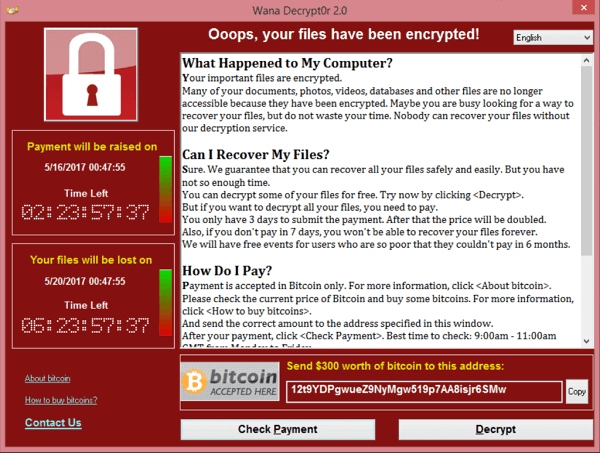
\includegraphics[scale=0.7]{imagenes/screenshot.png}
	\caption[Imagen que aparece en un ordenador infectado]{Imagen que aparece en un ordenador infectado}
\end{figure}
De todas las opciones que existen, los ataques de Ransomware, quizás sean los más rentables en términos económicos. Su único objetivo es secuestrar los datos de un ordenador para poder pedir un rescate por ellos. El uso de la criptografía y de las nuevas formas de pago, que garantizan el anonimato, son fundamentales para realizar un buen ataque.\\\\
El primer Ransomware que apareció, fue AIDS Trojan en 1989. Este malware escondía y cifraba los nombres de todos los ficheros que se encontrasen en el disco C. Esto hacia que el ordenador se quedase inservible, teniendo que pagar 189\$ a una oficina de correos en Panamá.\\\\
En 2011 apareció el primer Trojan, que se aprovechaba de la moda de los pagos anónimos como medio de pago del rescate de los datos. Actualmente, el uso de medios de pago anónimos es algo muy común, aunque no siempre es fácil para el atacante recuperar el dinero.\\\\
Según las últimas tendencias de Ransomware, el uso de criptografía simétrica es la forma más empleada para hacer que los datos no puedan recuperarse, a menos que se tenga la contraseña. Pero esto no siempre ha sido así, hubo un tiempo en el que la idea principal no era cifrar los datos de un ordenador, sino bloquearlo y hacer que su uso fuera limitado. Estos son los llamados "Lockers", que se valen de exploits y ciertas vulnerabilidades del sistema operativo anulando cualquier interacción con la máquina afectada.\\\\
Históricamente, este tipo de ataques ha estado siempre dirigido a ordenadores personales, por lo que los ordenadores con un sistema operativo de la familia Microsoft, eran más propensos a este tipo de ataque. Con la llegada de los Smartphone y la capacidad que tienen para ser ordenadores personales portátiles, en 2014 salió un Ransomware centrado en el sistema operativo Android. 

El desarrollo del proyecto en cuestión, se centrará en la presentación de una nueva herramienta creada para facilitar la protección de sistemas informáticos frente a ataques de Ransomware. La idea en la que se basará este trabajo, surgió al descubrir algo similar en el mercado. Una aplicación llamada Ransim. Ésta, ejecuta una serie de escenarios, los más comunes, intentando asemejarse a un programa de Ransomware real.\\\\
El objetivo, es llevar a cabo los procedimientos necesarios para que, dicha herramienta, sea capaz de realizar la misma función que la previamente descubierta, aunque con una diferencia, y es que esta nueva herramienta presentaría un código abierto con posibilidad de ejecutar escenarios ad hoc. Por este motivo, el nombre elegido, ha sido OpenRansim. OpenRansim podrá encontrarse en la siguiente URL: \href{https://github.com/iserranos/OpenRansim}{Github}. 
Al tratarse de una aplicación de código abierto, cualquier persona con un cierto interés en el tema, podrá colaborar en su desarrollo, lo cual, será clave y podrá favorecer al correcto funcionamiento de la misma.
 

%\section{Ransomware, historia y motivación del proyecto}
%\subsection{Introducción}


%\subsection{Historia}


\subsection{Motivación del proyecto}
Parece ser, que nos encontramos en un nuevo mundo, el mundo de la digitalización. En este nuevo mundo, uno de los elementos más valiosos, ha pasado a ser la disposición de datos y su control. Por este motivo, el Ransomware, se ha convertido, en la opción con más posibilidades de hacer negocio para los ciberdelincuentes.\\\\
A comienzos del año 2017, apenas se conocía la existencia de este tipo de ataques, hasta que saltó a la fama WannaCry. En Mayo del mismo año, se lanzó un ataque masivo que afectó a nivel mundial, incluyendo grandes empresas españolas. El 27 de Junio de 2017 salió a la luz otro Ransomware llamado NotPetya. Este último también se propagó a escala mundial afectando a Ucrania, Estados Unidos e Italia, principalmente.\\\\
Debido al notable aumento de este tipo de ataques, la existencia de una herramienta que pueda medir, de forma fiable, como de protegido se encuentra un ordenador frente a este tipo de amenazas, pasa a convertirse en un recurso vital para compañías de todo el mundo. 
OpenRansim, ha sido desarrollado, para que cualquier persona, sea capaz de cubrir sus necesidades de protección ante posibles ataques de Ransomware. 

\subsection{Contribuciones}

\section{OpenRansim}
\subsection{Introducción}
OpenRansim es una herramienta de línea de comando, desarrollada en Golang bajo la licencia GPL 3.0 de uso libre. La puesta en marcha, se ha llevado a cabo, mediante la utilización de 10 escenarios básicos, aunque su diseño, basado en módulos, permite la creación de escenarios nuevos, haciendo que sea personalizable.
\subsection{Pre task \& Post task}
Para comprobar que un escenario se ha ejecutado correctamente, y poder así dictaminar si existe una posibilidad de infección o no, se han añadido al desarrollo de la herramienta, las llamadas: pre-task y post-task. Antes de empezar a ejecutar un escenario, la herramienta crea una carpeta especifica donde se van a realizar las pruebas definidas por cada escenario. De esta forma se ejecuta la prueba bajo un entorno controlado sin que afecte a ningún archivo real.\\\\
Una vez ejecutado un escenario, es necesario comprobar si éste se ha completado correctamente o si, por el contrario, el sistema operativo ha interrumpido la ejecución, detectando y bloqueando, de esta manera, la posible acción maliciosa.  
\subsection{Escenarios}
Para esta primera versión de OpenRansim se han llevado a cabo una serie de escenarios, que intentan simular las ejecuciones de varios tipos de Ransomware. Para ello, se han estudiado cuales son las formas de funcionar de las familias de Ransomware más representativas. Estos son los 10 escenarios: 
\begin{itemize}
\item InsideCryptor – Cifra los datos y sobrescribe los archivos originales.
\item LockyVariant – Simula una de las incontables variables del Ransomware Locky.
\item Mover – Cifra los datos en una carpeta diferente a la original y elimina los ficheros originales.
\item Replacer – Reemplaza el contenido de los archivos.
\item Streamer – Cifra todos los datos y los agrupa en un único fichero.
\item StrongCryptor – Cifra los datos y borra los ficheros originales de forma segura.
\item StrongCryptorFast – Cifra los datos y borra los archivos originales.
\item StrongCrytptorNet – Cifra los datos, borra los ficheros originales y simula una conexión HTTP.
\item ThorVariant – Simula una de las incontables variables del Ransomware Thor.
\item WeakCryptor – Utiliza un cifrado débil para cifrar los datos y elimina los archivos originales.
\end{itemize}
\subsection{BYOS, Build Your Own Scenario}
Aquí se habla de como te puedes crear tu propio escenario.
\subsection{Implementación}
\section{Validación experimental}
\section{Trabajos relacionados}
\section{Conclusión}
No siempre se devuelven los archivos después de pagar
\appendix
\section{Planificación del proyecto}
\section{Presupuesto}

\end{document}
